\documentclass{beamer}
\usepackage{amsmath}
\usepackage{amssymb}
%\usepackage{asymptote}
\usepackage{calc}
%\usepackage{caption}
%\usepackage{chemfig}
\usepackage{color}
\usepackage{commath}
%\usepackage{enumitem}
\usepackage[c]{esvect}
%\usepackage{etoolbox}
\usepackage{fancyhdr}
%\usepackage{float}
%\usepackage{fontspec}    %fontspec only works with xetex and luatex.
%\usepackage{fp}
\usepackage{geometry}
\usepackage{graphicx}
\usepackage{lastpage}
%\usepackage{listings}
%\usepackage{luacode}
\usepackage{mathtools}
%\usepackage{mhchem}
%\usepackage{pgfplots}
%\usepackage{setspace}
\usepackage{siunitx}
%\usepackage{tcolorbox}
%\usepackage{tikz}

\title{Visualizing Data using t-SNE}
\author{Taran Lynn, Xiaoli Yang, Xiaoxin Chen}

\begin{document}
\maketitle

\begin{frame}
  \frametitle{Data Visualization and Manifold Learning}

  \begin{enumerate}
  \item What is the goal of data visualization?

    \pause

  \item We want to preserve as much structure between data points when
    mapping to a lower dimension.

  \item What is the ideal case when reducing to 2D from a higher dimension?
  \end{enumerate}

  \pause

  \begin{figure}
    \centering
    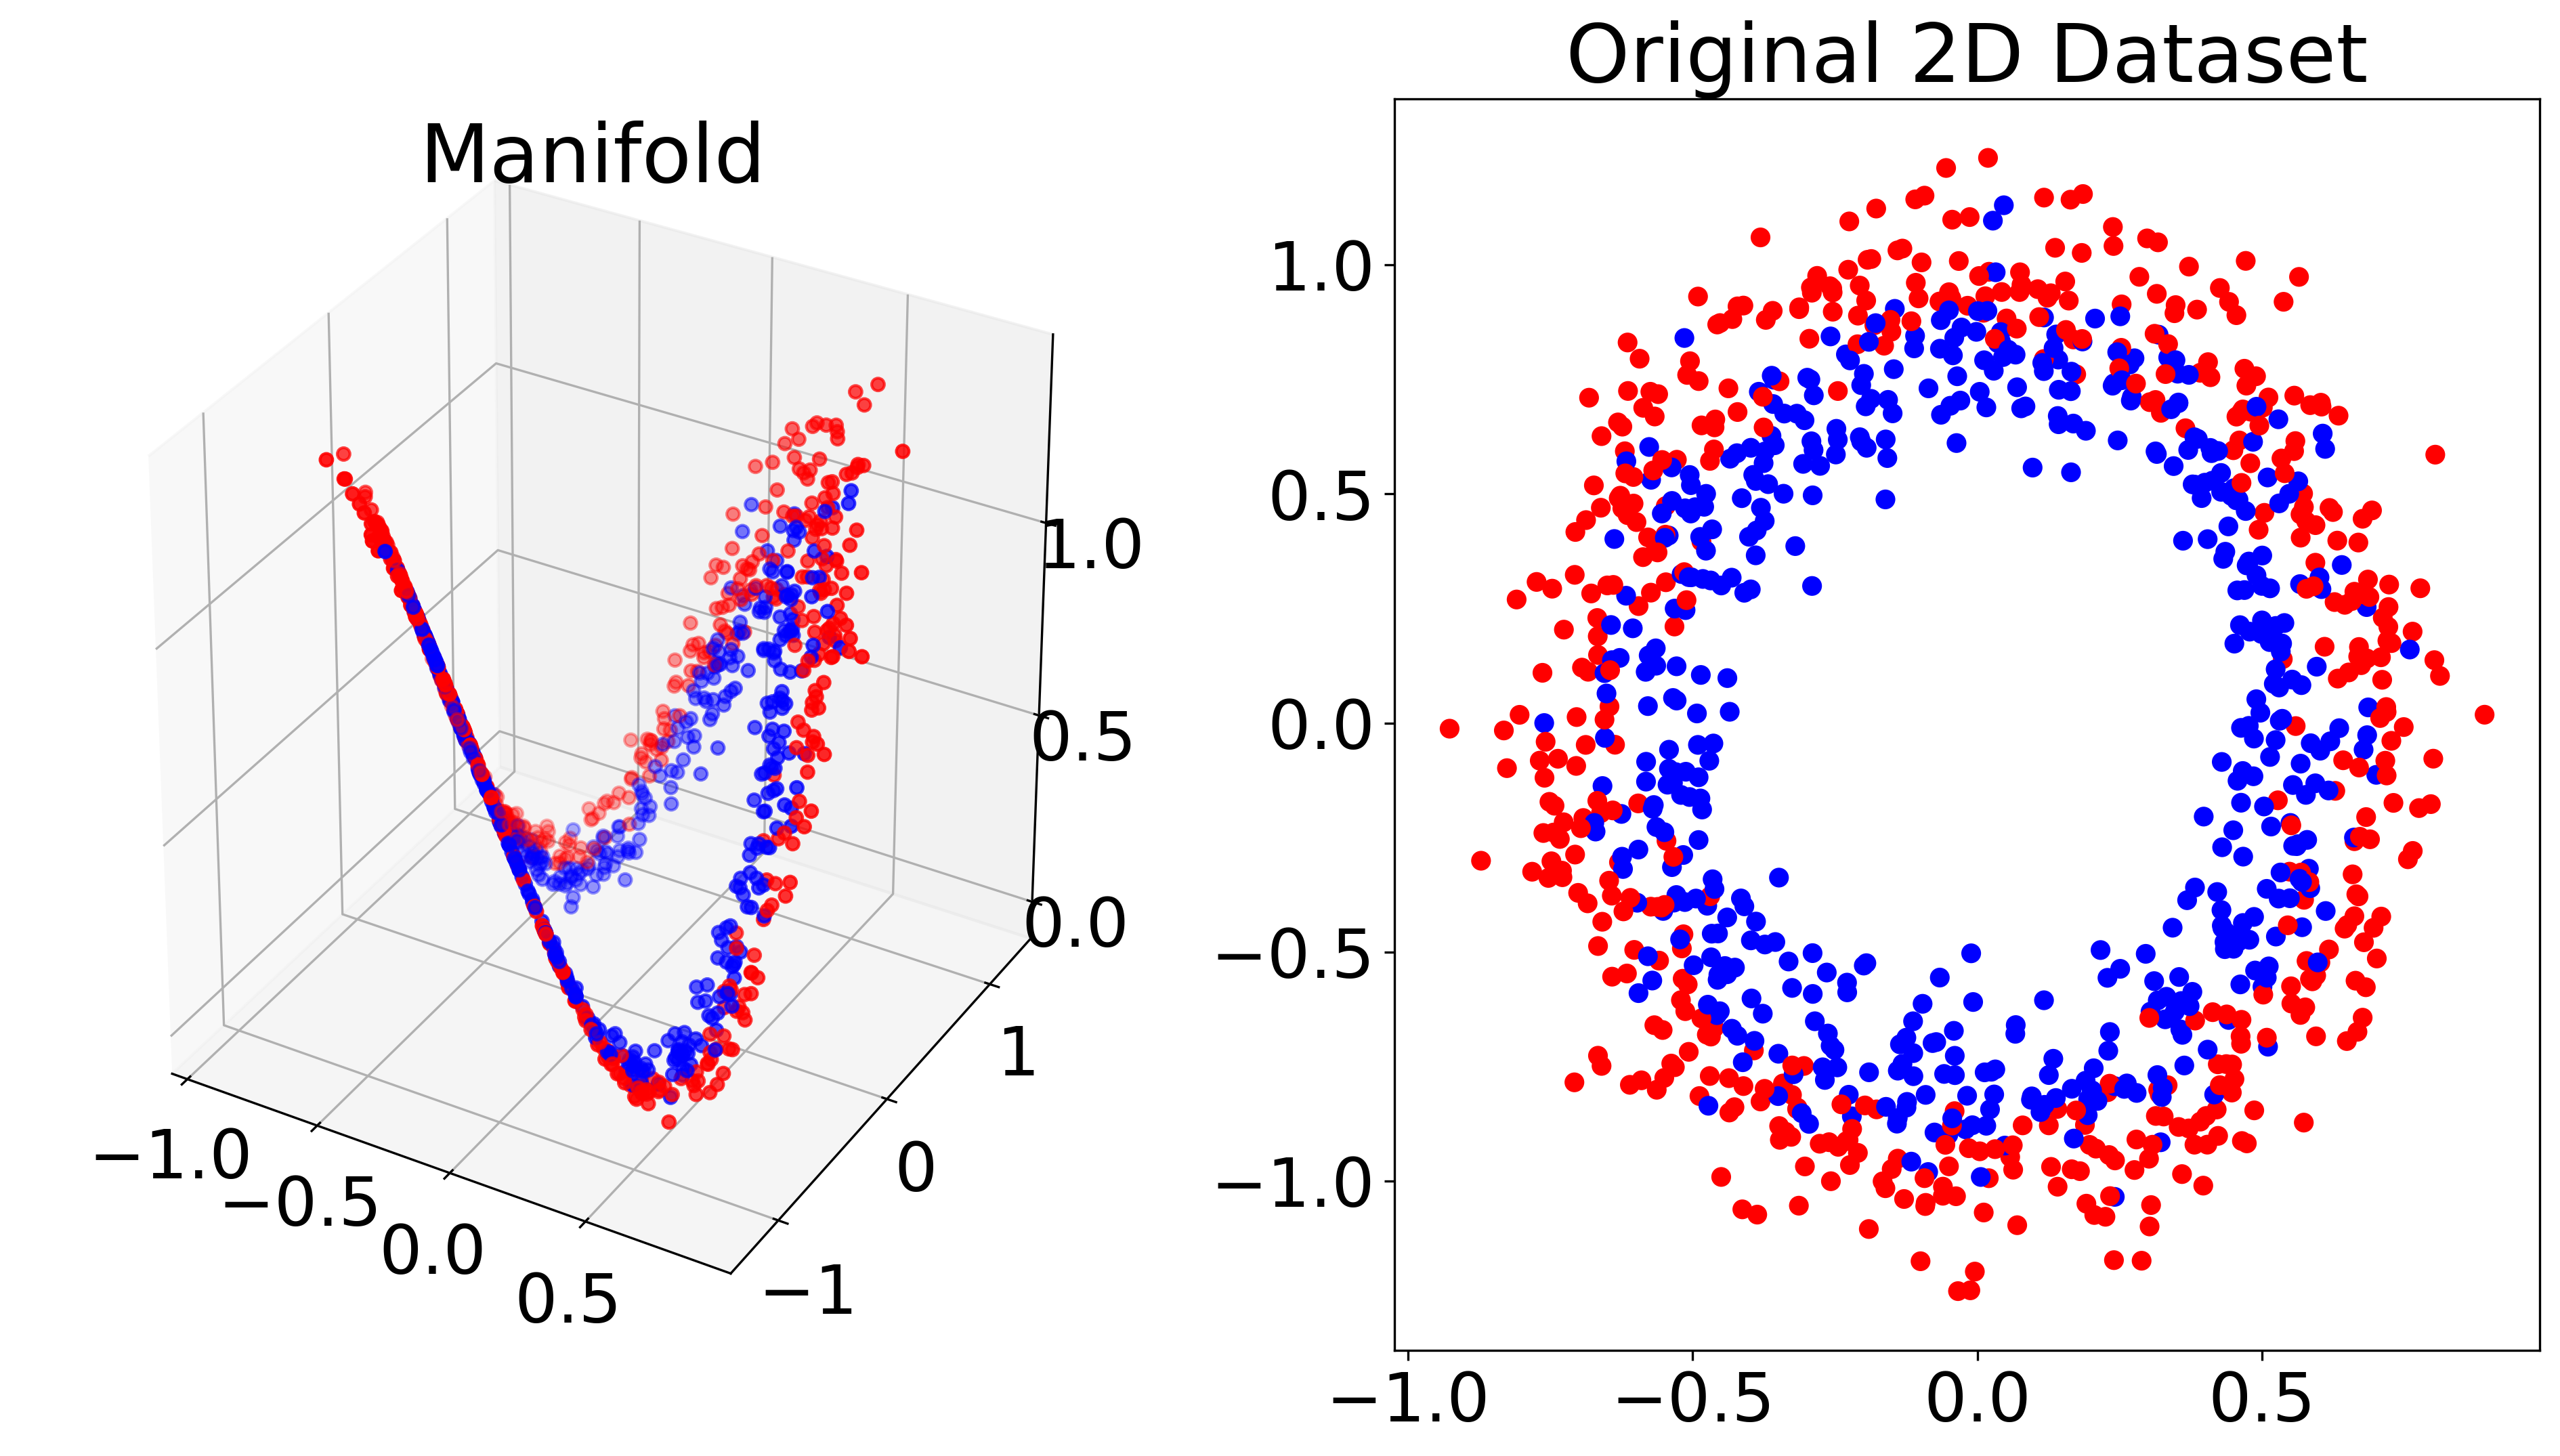
\includegraphics[height=0.5\textheight]{images/manifold/manifold.png}
  \end{figure}
\end{frame}

\begin{frame}
  \frametitle{Stochastic Neighbor Embedding (SNE)}
  \framesubtitle{Spring Metaphor}

  \begin{enumerate}
  \item Consider putting a spring between each point in
    higher-dimensional space, and then squashing the points down into a
    lower dimension.

  \item Spring tension is given by neighbor locality.
  \end{enumerate}

  \begin{figure}
    \centering
    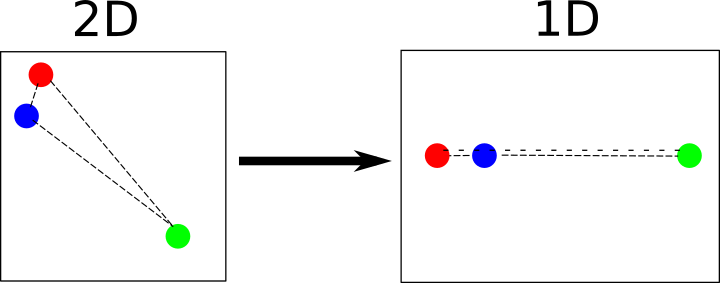
\includegraphics[width=\linewidth]{images/spring.png}
  \end{figure}
\end{frame}

\begin{frame}
  \frametitle{Stochastic Neighbor Embedding (SNE)}
  \framesubtitle{What is $p_{j|i}$?}

  \begin{enumerate}
  \item $p_{j|i} = \frac{\exp\del{-|| x_i - x_j ||^2/2\sigma_i^2}}{\sum_{k \neq i} \exp\del{-|| x_i - x_k ||^2/2\sigma_i^2}}$
  \item Probability datapoint $x_i$ views $x_j$ as its neighbor given Gaussian with variance $\sigma_i$
  \end{enumerate}

  \begin{figure}
    \centering
    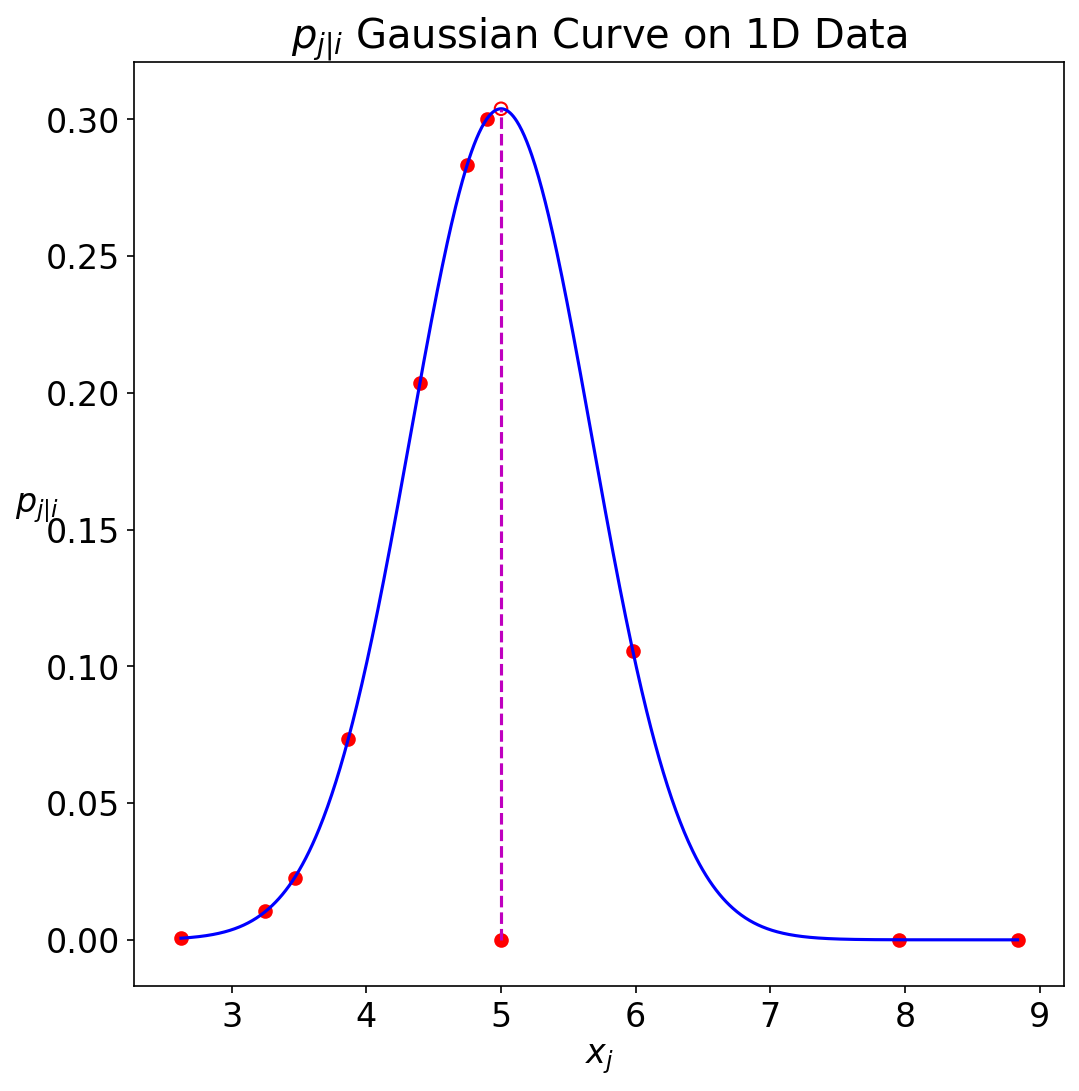
\includegraphics[width=0.5\linewidth]{images/gauss/gauss.png}
  \end{figure}
\end{frame}

\begin{frame}
  \frametitle{Stochastic Neighbor Embedding (SNE)}
  \framesubtitle{Determining $\sigma_i$}

  \begin{center}
    \small
    
    \begin{tabular}{ll}
      Perplexity & Smooth approximation of number of neighbors\\
      & $Perp(P_i) = 2^{H(P_i)}$\\
      \hline
      Shannon Entropy & Information present in probability space\\
      & $H(P_i) = -\sum_j p_{j|i} \log_2{p_{j|i}}$\\
    \end{tabular}
  \end{center}
  
  \begin{figure}
    \centering
    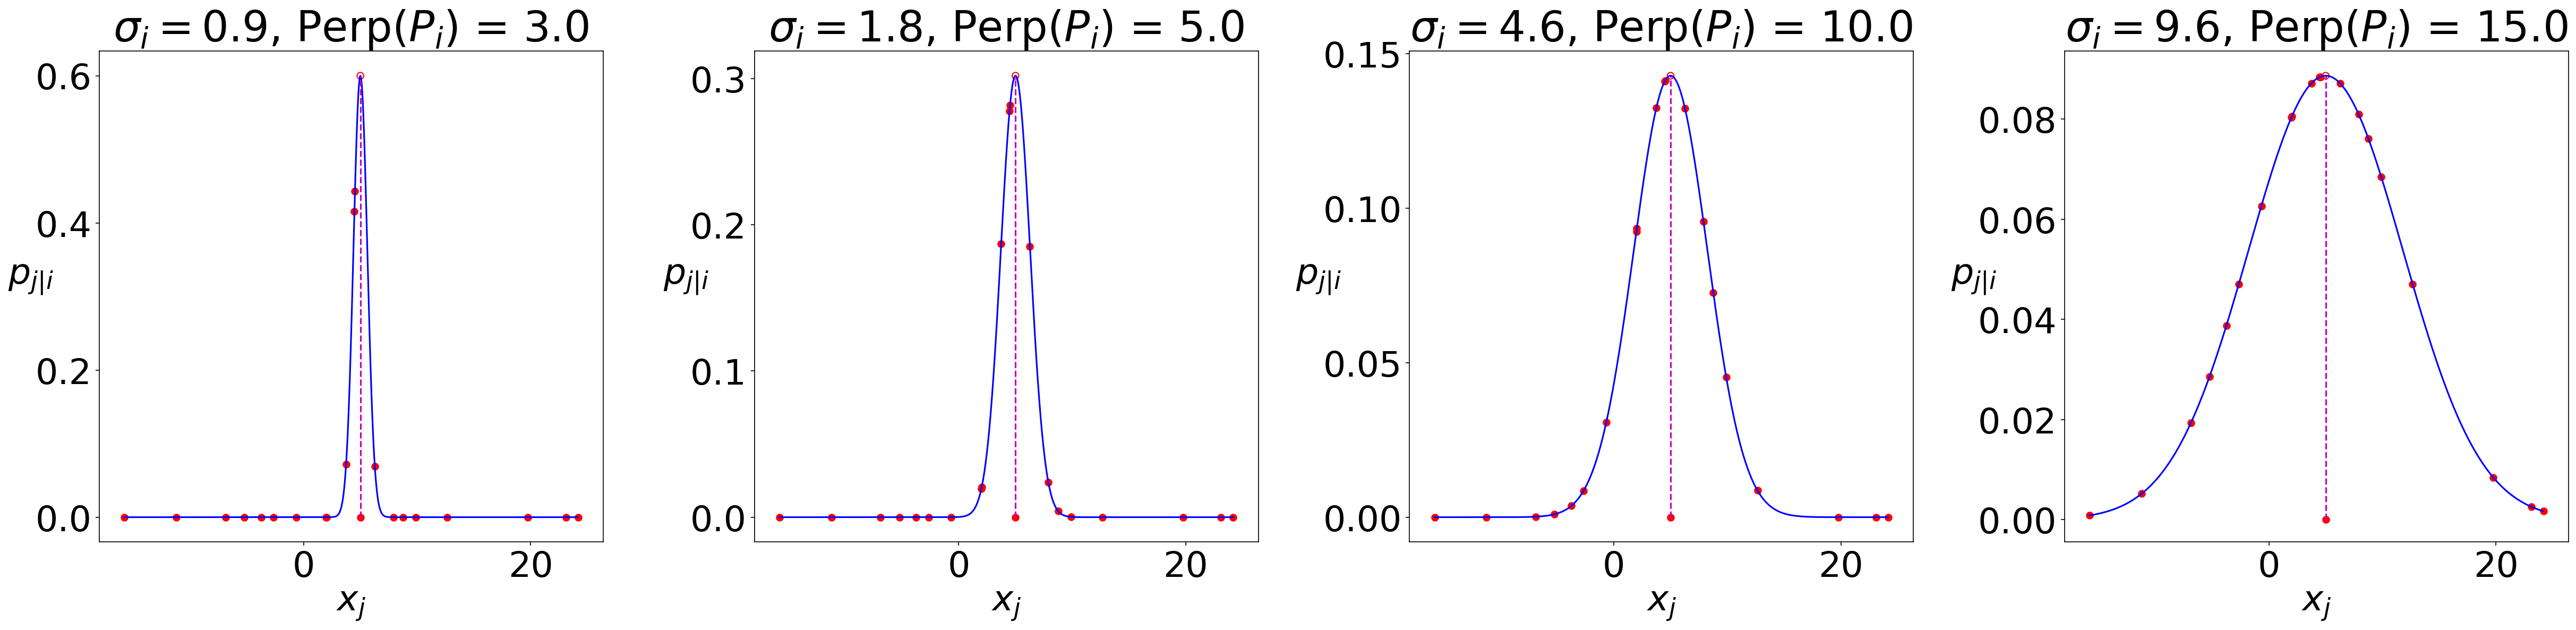
\includegraphics[height=0.6\textheight]{images/perp/perp.png}
  \end{figure}
\end{frame}

\begin{frame}
  \frametitle{Stochastic Neighbor Embedding (SNE)}
  \framesubtitle{Gradient Descent Optimization}

  \begin{enumerate}
  \item $q_{j|i}$ is analogous to $p_{j|i}$ for lower dimension points $y_i$ and $y_j$.
    $\sigma = 1/\sqrt{2}$ for all $q_{j|i}$

  \item Cost function is $C = \sum_i KL(P_i || Q_i) = \sum_i \sum_j p_{j|i} \log\frac{p_{j|i}}{q_{j|i}}$

  \item $\pd{C}{y_i} = 2 \sum_j \del{p_{j|i} - q_{j|i} + p_{i|j} - q_{i|j}} \del{y_i - y_j}$

  \item $Y^{(t)} = Y^{(t - 1)} + \nu \pd{C}{Y} + \alpha(t) \del{Y^{(t - 1)} - Y^{(t - 2)}}$

    \item Simulated annealing through decaying Gaussian noise
  \end{enumerate}
\end{frame}

\begin{frame}
  \frametitle{Problems with SNE}

  \begin{itemize}
  \item Computational inefficiency

  \item Overcrowding
  \end{itemize}
\end{frame}

\end{document}
